%%%%%%%%%%%%%%%%%%%%%%%%%%%%%%%%%%%%%%%%%
% fphw Assignment
% LaTeX Template
% Version 1.0 (27/04/2019)
%
% This template originates from:
% https://www.LaTeXTemplates.com
%
% Authors:
% Class by Felipe Portales-Oliva (f.portales.oliva@gmail.com) with template 
% content and modifications by Vel (vel@LaTeXTemplates.com)
%
% Template (this file) License:
% CC BY-NC-SA 3.0 (http://creativecommons.org/licenses/by-nc-sa/3.0/)
%
%%%%%%%%%%%%%%%%%%%%%%%%%%%%%%%%%%%%%%%%%

%----------------------------------------------------------------------------------------
%	PACKAGES AND OTHER DOCUMENT CONFIGURATIONS
%----------------------------------------------------------------------------------------

\documentclass[
	12pt, % Default font size, values between 10pt-12pt are allowed
	%letterpaper, % Uncomment for US letter paper size
	%spanish, % Uncomment for Spanish
]{fphw}

% Template-specific packages
\usepackage[utf8]{inputenc} % Required for inputting international characters
\usepackage[T1]{fontenc} % Output font encoding for international characters
\usepackage{mathpazo} % Use the Palatino font

\usepackage{graphicx} % Required for including images

\usepackage{booktabs} % Required for better horizontal rules in tables

\usepackage{listings} % Required for insertion of code

\usepackage{enumerate} % To modify the enumerate environment

\usepackage{float} %设置图片浮动位置的宏包
\usepackage{subfigure} %插入多图时用子图显示的宏包
\usepackage{ctex}
\usepackage{amsmath}
\usepackage{mathrsfs}

%----------------------------------------------------------------------------------------
%	ASSIGNMENT INFORMATION
%----------------------------------------------------------------------------------------

\title{Homework \#1} % Assignment title

\author{Chengqi Liu (1954148), Maitraiyi Dandekar (1990136),\\ Zakariae Jabbour (2039702)} % Student name

\date{September 12th, 2023} % Due date

\institute{Eindhoven University of Technology} % Institute or school name

\class{Cryptology (2MMC10)} % Course or class name

\professor{Tanja Lange} % Professor or teacher in charge of the assignment

%----------------------------------------------------------------------------------------

\begin{document}

\maketitle % Output the assignment title, created automatically using the information in the custom commands above

%----------------------------------------------------------------------------------------
%	ASSIGNMENT CONTENT
%----------------------------------------------------------------------------------------
\textbf{1.}\\
Use Python programming to solve this problem.\\
\begin{figure}[H] 
	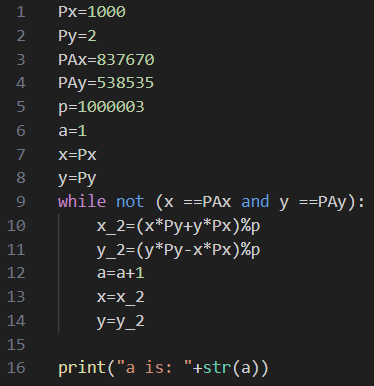
\includegraphics[width=0.5\textwidth]{1.png}
\end{figure}
Run the program and it gives the result "a is: 271828".\\
Therefore, we find the integer $a=271828$ with $P_A=aP$.\\
You can find this program in the file "Question1.py".\\
\textbf{2.}\\
\textbf{Show:\\}
\[(x_1,y_1)+(x_2,y_2)=(\frac{x_1y_2+x_2y_1}{1+dx_1y_1x_2y_2},\frac{y_1y_2-x_1x_2}{1-dx_1y_1x_2y_2})\]
$\forall P=(x,y)\in x^2+y^2=1+dx^2y^2$:
\begin{align*}
	P+(0,1)=&(\frac{1x+0y}{1+0dxy},\frac{y-0x}{1-0dxy})=(x,y)=P\\
	(0,1)+P=&(\frac{0y+1x}{1+0dxy},\frac{y-0x}{1-0dxy})=(x,y)=P
\end{align*}
So. $P+(0,1)=(0,1)+P=P$. $(0,1)$ is the neutral element with respect to the addition law on an Edwards curve.\\
$\forall P=(x,y)\in x^2+y^2=1+dx^2y^2$:
\begin{align*}
	2P=&(\frac{2xy}{1+dx^2y^2},\frac{y^2-x^2}{1-dx^2y^2})
\end{align*}
So,
\begin{align*}
	2(0,-1)=&(\frac{0}{1+0},\frac{1-0}{1-0})=(0,1)\\
	4(\pm1,0)=&2(\frac{0}{1+0},\frac{0-1}{1-0})=2(0,-1)=(0,1)\\
\end{align*}
So, $(0,-1)$ has order 2 and $(\pm1,0)$ have order 4.\\
\textbf{3.}\\
\textbf{Show:\\}
First check the existence of the points $(\pm b,\pm b), b\in\mathbb{R}$.
\begin{align*}
	&\exists(\pm b,\pm b)\in x^2+y^2=1+dx^2y^2\\
	\Leftrightarrow&2b^2=1+db^4 \text{ has a solution}\\
	\Leftrightarrow&db^4-2b^2+1=0 \text{ has a solution}
\end{align*}
Let $x=b^2\geq0$, $f(x)=dx^2-2x+1$. So $f(x)$ is a quadratic function. It equals $f(x)=0$ having a solution. By the definition of Edwards curve, $d\not\in\{0,1\}$.\\
When $d<0$, according to the properties of quadratic functions, $\lim\limits_{x\to+\infty}f(x)=-\infty$, $f(0)=1>0$. So, there must be a solution in $(0,+\infty)$.\\
When $d>0$, $f_{min}(x)=f(\frac{1}{d})=\frac{d-1}{d}$. Because $f_{min}(x)\leq0$ and $d\not\in\{0,1\}$, we get $d\in(0,1)$.\\
So, when $d\in(-\infty,0)\cup(0,1)$, the points $(\pm b,\pm b), b\in\mathbb{R}$ exist.\\
\\
Second, show they have order 8:\\
Because $(\pm b,\pm b)\in x^2+y^2=1+dx^2y^2$, $2b^2=1+db^4$.\\
If $1-db^4=0$, $d=\frac{1}{b^4}$. 
\begin{align*}
	&2b^2=1+db^4\\
	\Rightarrow&2b^2=2\\
	\Rightarrow&b=\pm1\\
	\Rightarrow&d=1
\end{align*}
But we have $d\not\in\{0,1\}$. It's a contradiction. So, $1-db^4\not=0$.
\begin{align*}
	2(\pm b,\pm b)=&(\frac{2b^2}{1+db^4},\frac{0}{1-db^4})\\
	=&(\frac{2b^2}{1+db^4},0)\\
	=&(\frac{2b^2}{2b^2},0)\\
	=&(1,0)
\end{align*}
From the question 2, we have shown that $(1,0)$ has order 4. $4(1,0)=(0,1)$. So,
\begin{align*}
	8(\pm b,\pm b)=&4(2(\pm b,\pm b))\\
	=&4(1,0)\\
	=&(0,1)
\end{align*}
In all, when $d\in(-\infty,0)\cup(0,1)$, the points $(\pm b,\pm b), b\in\mathbb{R}$ exist, and have order 8.
\end{document}
